\documentclass{beamer}
\usepackage{beamerthemeshadow}
\usepackage[brazil]{babel}
\usepackage[utf8]{inputenc}
\usepackage{graphicx}
\usepackage[compatibility=false]{caption}
\usepackage{subcaption}

\begin{document}
\title{MC920: Introdução ao Processamento de Imagem Digital}
\author{Martin de Oliveira (118077) \and Rafael Hermano (121286)}
\date{\today}

\frame{\titlepage}

\frame{\frametitle{Dilatação geodésica}
    \[
        \delta^1_X(Y) = \delta_B(Y) \cap X
    \]
    \[
        \delta^n_X(Y) = \delta^1_X(\delta^1_X(\cdots\delta^1_X(Y)))
    \]
    \begin{figure}[!ht]
        \centering
        \begin{subfigure}[ht]{0.25\textwidth}
            \fbox{
\includegraphics[width=\textwidth]{image.png}}
            \caption{Original}
        \end{subfigure}
        \qquad
        \begin{subfigure}[ht]{0.25\textwidth}
            \fbox{
\includegraphics[width=\textwidth]{mask.png}}
            \caption{Máscara}
        \end{subfigure}
        \qquad
        \begin{subfigure}[ht]{0.25\textwidth}
            \fbox{
\includegraphics[width=\textwidth]{geodesic_dilation.png}}
            \caption{Dilatação geodésica}
        \end{subfigure}
    \end{figure}
}

\frame{\frametitle{Reconstrução Geodésica}
    \[
        \delta^1_f(g) = min(\delta_1(g),f)
    \]
    \[
        \delta^n_f(g) = \delta^1_f(\delta^1_f(\cdots\delta^1_f(g)))
    \]
    \vfill
    \[
        \text{máscara } \rightarrow f = \left[\text{\texttt{ 0 0 1 3 3 7 7 7 7 5 2 1 1 }}\right]
    \]
    \[
        \text{marcador } \rightarrow g = \left[\text{\texttt{ 0 0 1 2 2 2 5 2 2 2 2 1 1 }}\right]
    \]
    \vfill
    \[ \delta^1_f(g) = \left[\text{\texttt{ 0 0 1 3 3 3 6 3 3 3 2 1 1}}\right] \]
    \[ \delta^2_f(g) = \left[\text{\texttt{ 0 0 1 3 3 3 6 3 3 3 2 1 1}}\right] \]
}


\frame{\frametitle{Segmentação morfológica}
    \begin{figure}[!ht]
        \centering
        \begin{subfigure}[ht]{0.41\textwidth}
            \fbox{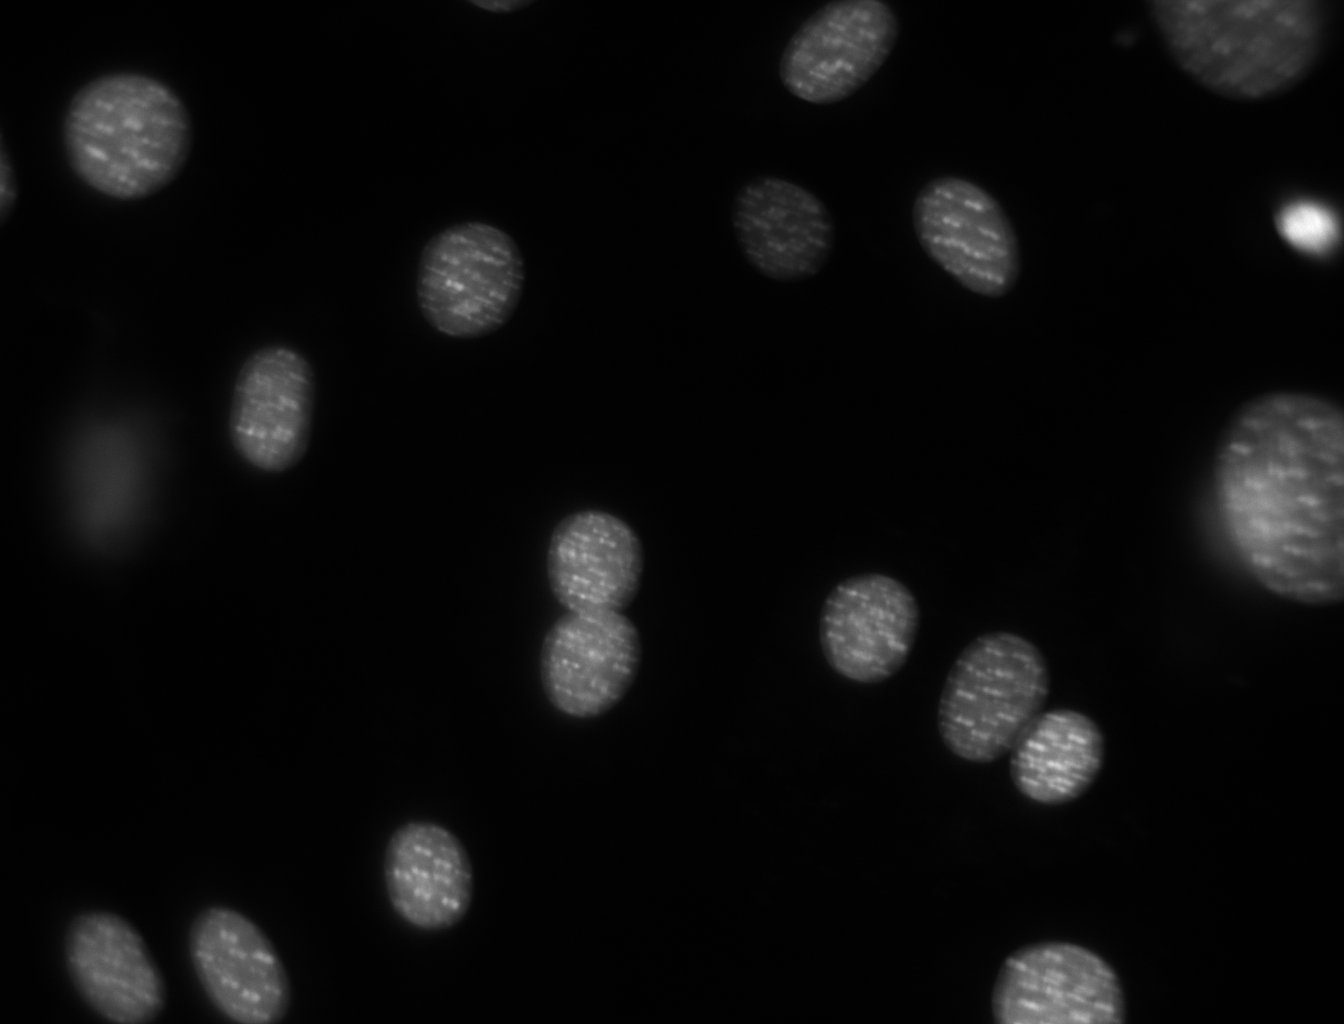
\includegraphics[width=\textwidth]{dna.jpeg}}
        \end{subfigure}
        \qquad
        \begin{subfigure}[ht]{0.41\textwidth}
            \fbox{
\includegraphics[width=\textwidth]{dnaf.jpeg}}
        \end{subfigure}
        \\
        \begin{subfigure}[ht]{0.41\textwidth}
            \fbox{
\includegraphics[width=\textwidth]{dist.jpeg}}
        \end{subfigure}
        \qquad
        \begin{subfigure}[ht]{0.41\textwidth}
            \fbox{
\includegraphics[width=\textwidth]{watershed.jpeg}}
        \end{subfigure}
    \end{figure}
}
\end{document}
